\documentclass[letterpaper, reqno,11pt]{article}
\usepackage[margin=1.0in]{geometry}
\usepackage{color,latexsym,amsmath,amssymb,graphicx, float}
\usepackage{hyperref}

\hypersetup{
colorlinks=true,
linkcolor=magenta,
filecolor=magenta,
urlcolor=cyan,
}

\graphicspath{ {images/} }

\newcommand{\RR}{\mathbb{R}}
\newcommand{\CC}{\mathbb{C}}
\newcommand{\ZZ}{\mathbb{Z}}
\newcommand{\QQ}{\mathbb{Q}}
\newcommand{\NN}{\mathbb{N}}
\newcommand{\st}{\text{ s.t.}\ }

\begin{document}
\pagenumbering{arabic}
\title{Math 305 Homework 1}
\date{12/01/22}
\author{Xander Naumenko}
\maketitle

{\noindent\bf 1a.} Expanding:

\[
    (1+i)(3-2i)(2+3i)=(3+2+3i-2i)(2+3i)=(5+i)(2+3i)
\] 

\[
    =10-3+2i+15i=7+17i
.\] 

{\noindent\bf 1b.} Expanding: 

\[
    (\frac{1+i}{2+i})^2=(\frac{(1+i)(2-i)}{4+1})^2=\frac{1}{25}(3+i)^2=\frac{8}{25}+\frac{6i}{25}
.\] 


{\noindent\bf 1b.} Expanding: 

\[
    (1+i)^8=(\sqrt{2} e^\frac{\pi}{4})^8=(\sqrt{2} )^8=16
.\] 

{\noindent\bf 2.} Let $z=a+bi$ with $|z|=1$. Then we have that 

\[
Re(\frac{1}{1-z})=Re(\frac{1-a+bi}{(1-a-bi)(1-a+bi)})=Re(\frac{1-a+bi}{1+a^2-2a+b^2})=Re(\frac{1-a}{1-2a+1})=\frac{1}{2}
.\] 

Note that the second to last step used the fact that $a^2+b^2=1$ since $|z|=1$. 

{\noindent\bf 3a.} Note that $ \sqrt{3} +i=\frac{1}{4}e^{\frac{\pi}{6}}$, so $|\sqrt{3} +i|=|\sqrt{3} -i|=\frac{1}{4}$. Thus we have that 

\[
\bigg|\frac{(\sqrt{3}+i)^{100}}{(\sqrt{3}-i)^{100}}\bigg|=|\frac{4}{4}|=1
.\] 

{\noindent\bf 3b.} Using the formula for the (capital A) argument with the appropriate quadrant, we get 

\[
Arg(-1-\sqrt{3} i)=-\pi+\arctan(\frac{\sqrt{3} }{1})=-\frac{2\pi}{3}
.\] 

{\noindent\bf 3c.} Using the same process as previous question except adding an additional periodic term: 

\[
arg(1-\sqrt{3} i)=\arctan(\frac{\sqrt{3} }{1})+2\pi n=-\frac{\pi}{3}+ 2\pi n, n\in\ZZ
.\] 

{\noindent\bf 3d.} Expanding:

\[
arg(-1+2i)=\arctan(-2)+2\pi n, n\in\ZZ
.\] 

{\noindent\bf 4a.} The principal argument of the number geometrically is $\frac{3\pi}{4}$. Writing it in polar form uses this angle along with its magnitude to get $3\sqrt{2}e^{\frac{3}{4}\pi i}$. 

{\noindent\bf 4b.} Writing the numerator and denominator in polar coordinates and dividing, we get 

\[
    \frac{1-i}{-\sqrt{3} +i}=\frac{\sqrt{2} e^{-\frac{\pi}{4}}}{4e^{\frac{5\pi}{6}}}=\frac{1}{\sqrt{2} }e^{\pi i \frac{13}{12}}=\frac{1}{\sqrt{2} }e^{-\pi i \frac{11}{12}}
.\] 

Thus the principal argument is $\frac{11}{12}$. 

{\noindent\bf 4c.} Writing the number first in polar form then squaring, we get 

\[
    (\sqrt{3} -i)^2=(2e^{-\frac{\pi}{6}i})^2=4e^{-\frac{\pi}{3}i}
.\] 

Thus the principal argument is $-\frac{\pi}{3}$

{\noindent\bf 5a.} This is note true, for example consider the case that $Arg(z_1)=Arg(z_2)=\frac{3\pi}{4}$. Then it can't be that $Arg(z_1z_2)=\frac{3\pi}{2}$ so the identity can't hold. 

{\noindent\bf 5b.} The statement is true. Taking the conjugate reflects the original number accross the real axis, which corresponds with the negative of the angle (barring the case where the number is a negative real number, which wasn't included in the question). 

{\noindent\bf 5c.} This statement is true. For all non real numbers this is true as a consequence of the previous part. For real numbers, this is true since $arg(z)=\pi+2\pi n=-\pi+2\pi n=-arg(\overline{z})$ for the case where $z$ is negative and real. 

{\noindent\bf 5d.} This is true by the definition of $arg(z)$. 

{\noindent\bf 6a.} Expanding with De Moivre's formula, we get 

\[
i\sin(3\theta)=((\cos\theta+i\sin\theta)^3-\cos(3\theta))
.\] 

The real part must go to zero, so we only care about the imaginary part:

\[
i\sin(3\theta)=3i\sin\theta\cos^2\theta-i\sin^3\theta=3i\sin\theta-3i\sin^2\theta-i\sin^3\theta
.\] 

\[
=3i\sin\theta-4i\sin^3\theta
.\] 

Dividing by $i$ gives the required result. 

{\noindent\bf 6b.} Rewriting as exponentials, we have 

\[
\sum_{k=0}^{n} \cos k\theta=\sum_{k=0}^{n} \frac{1}{2}\left( e^{ik\theta}+e^{-ik\theta} \right) 
.\] 

Applying the geometric series, this becomes

\[
=\frac{1}{2}\left( \frac{1-e^{i(n+1)\theta}}{1-e^{i\theta}}+\frac{1-e^{-i(n+1)\theta}}{1-e^{-i\theta}} \right)=\frac{1}{2}\left( -\frac{e^{-i\frac{1}{2}\theta}-e^{i(n+\frac{1}{2}})\theta}{e^{i\frac{1}{2}\theta}+e^{ i \frac{1}{2}\theta}} +\frac{e^{i\frac{1}{2}\theta}-e^{-i(n+\frac{1}{2}})\theta}{e^{i\frac{1}{2}\theta}-e^{ i \frac{1}{2}\theta}}\right) 
.\] 
\[
=\frac{1}{2}+\frac{e^{i(n+\frac{1}{2}\theta}-e^{-i(n+\frac{1}{2}\theta}}{e^{i\frac{\theta}{2}}-e^{-i\frac{\theta}{2}}}=\frac{1}{2}+\frac{\sin(n+\frac{1}{2})\theta}{\sin(\frac{\theta}{2})}
.\] 

% {\noindent\bf 6b.} Rewriting using De Moivre's formula and omitting any terms with imaginary components since these must cancel out to zero (since the original component we started with is real), we get 

% \[
% \sum_{k=0}^{n} \cos k\theta=Re\left(\sum_{k=0}^{n}\left(\cos\theta+i\sin\theta\right)^{k}\right)
% .\] 

% Applying the geometric formula, we get 

% \[
% =Re\left(\frac{1-(\cos\theta+i\sin\theta)^{n+1}}{1-\cos\theta-i\sin\theta}\right)=Re \left( \frac{1-e^{i(n+1)\theta}}{1-e^{i\theta}} \right) =Re \left( \frac{\left(1-e^{i(n+1)\theta}\right)\left(1-e^{-i\theta}\right)}{2-e^{i\theta}-e^{-i\theta}} \right) 
% .\] 

% \[
% =Re \left( \frac{\left(1-e^{i(n+1)\theta}\right)\left(1-e^{-i\theta}\right)}{2-2\cos\theta} \right) 
% .\] 

% Because the denominator is real we can take just the real part of the numerator safely: 

% \[
% =\frac{1-e^{-i\theta}-e^{i(n+1)\theta}+e^{in\theta}}{2-2\cos\theta}=\frac{1-\cos\theta-\cos(n+1)\theta+\cos n\theta}{2-2\cos\theta}=\frac{1}{2}
% .\] 

{\noindent\bf 7a.} Expanding using the formula derived in class with $m=3$: 

\[
\int_{0}^{2\pi}\cos^{6}\theta d\theta=\frac{1}{2^{2m}}C_{2m}^{m}2\pi=\frac{1}{8\cdot 8}20\cdot 2\pi=\frac{5}{8}\pi
.\] 

{\noindent\bf 7b.} First do a change of variables, using $\theta^\prime=2\theta$:

\[
\int_0^{4\pi}\sin^{6}(2\theta) d\theta=\frac{1}{2}\int_0^{4\pi}\sin^{6}(\theta^\prime) d\theta^\prime=\frac{1}{2^{2m}}C_{2m}^{m}2\pi=\frac{5}{8}\pi
.\] 

{\noindent\bf 8a.} Let $z=x+iy$. Then using the definition of magnitude, we get 

\[
|z-1-i|^2=(x-1)^2+(y-1)^2=x^2+(y+2)^2
.\] 

\[
-2x+1-6y-3=0\implies y=-\frac{1}{3}x-\frac{1}{3}
.\] 

Thus the resultant shape is a line. 

{\noindent\bf 8b.} Let $z=x+iy$. Then we get that 

\[
|z|^2=x^2+y^2=(2|z+1|)^2=4(x+1)^2+4y^2\implies 0=3x^2+3y^2+8x+1
.\] 

\[
\implies 3(x-\frac{8}{6})^2+3y^2=\frac{4}{3}\implies (x-\frac{8}{6})^2+y^2=\frac{4}{9}
.\] 

This is the equation for a circle shifted in the x direction by $\frac{4}{3}$ with radius $\frac{10}{9}$. 

{\noindent\bf 8c.} Geometrically, note that this describes the set of all points for whom the sum of the distance between $(1, 0)$ and $(-1, 0)$ is equal to 4. This is the definition of an ellipse, from which simple geometry shows that the two major dimensions are $a=\sqrt{3} $ and $b=2$. Thus the equation for the resulting shape is 

 \[
\left( \frac{x}{\sqrt{3} } \right)^2 +\left( \frac{y}{2 } \right)^2 =1
.\] 

{\noindent\bf 9.} To find the final upper bound, we first find the lower bound of $|z-5|$. To do this first note that $|z-5|\geq ||z|-5|$. Also, using the condition given to use, we have that 

 \[
|z-1|\leq 1\implies | |z|-1 |\leq 1\implies |z| \leq 2
\] 

(we can get rid of the absolute value in the last step since the only way that that wouldn't be valid is if $|z|<1$ which is an even stronger statement than $|z|\leq 2$ ). Putting these two statements together we get that $|z-5|\geq ||z|+5|\geq 5-3=3$. Using this we have that 

 \[
\left| \frac{1}{z-5} \right| \leq \frac{1}{3}
.\] 

{\noindent\bf 10a.} Expanding with Euler's identity, we get 

\[
z(t)=2e^{it}=2\cos t+2i\sin t
.\] 

Because $|z(t)|=2\forall t$ of the above definition showing it goes through the entire span of the circle over $0\leq t\leq 2 \pi$, it must be a circle of radius 2. You can see the sketches in figure \ref{fig:q10}. part a is shifted upwards by 1 in the imaginary direction since you add $i$ to it, while the second one spirals since if you expand you get an exponential $e^{t}$ term in front which causes the line to grow as rotates around. 

\begin{figure}[htpb]
    \centering
    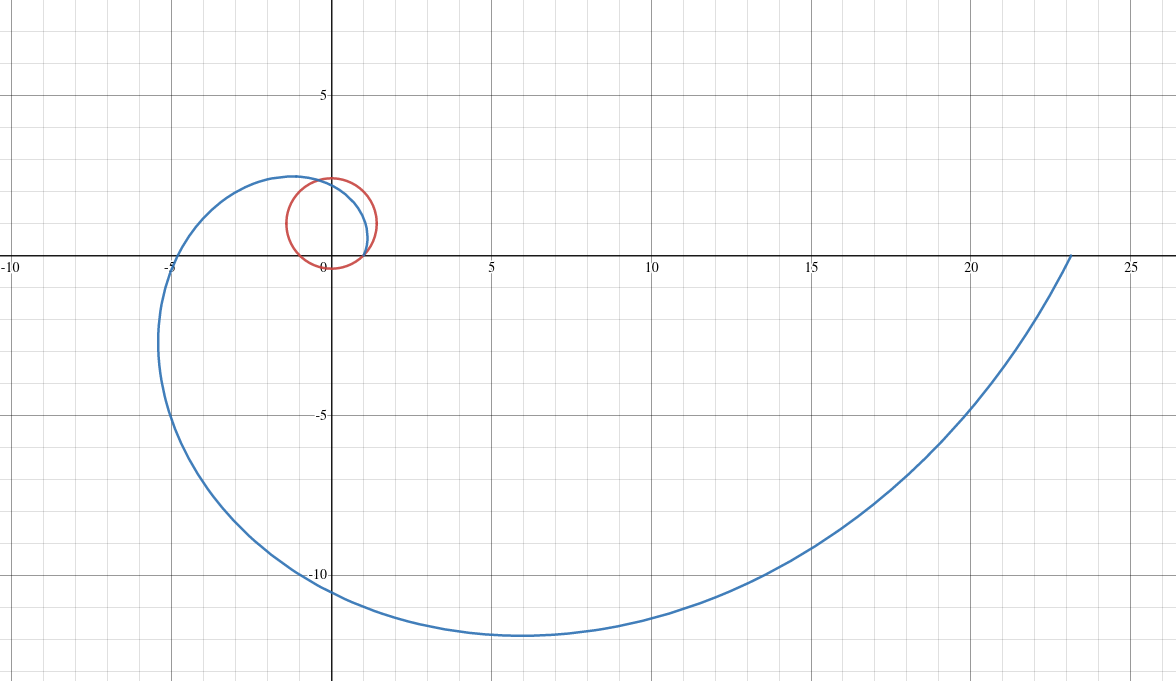
\includegraphics[width=0.8\textwidth]{q10}
    \caption{Sketchs for question 10. The red circle is part a and the blue line is part b. }
    \label{fig:q10}
\end{figure}

\end{document}
